
%%%%%%%%%%%%%%%%%%%%%%% file typeinst.tex %%%%%%%%%%%%%%%%%%%%%%%%%
%
% This is the LaTeX source for the instructions to authors using
% the LaTeX document class 'llncs.cls' for contributions to
% the Lecture Notes in Computer Sciences series.
% http://www.springer.com/lncs       Springer Heidelberg 2006/05/04
%
% It may be used as a template for your own input - copy it
% to a new file with a new name and use it as the basis
% for your article.
%
% NB: the document class 'llncs' has its own and detailed documentation, see
% ftp://ftp.springer.de/data/pubftp/pub/tex/latex/llncs/latex2e/llncsdoc.pdf
%
%%%%%%%%%%%%%%%%%%%%%%%%%%%%%%%%%%%%%%%%%%%%%%%%%%%%%%%%%%%%%%%%%%%


%\documentclass[runningheads,a4paper]{llncs}
\documentclass[journal]{IEEEtran}
\usepackage{amssymb}
\usepackage{amsmath}
\setcounter{tocdepth}{3}
\usepackage{graphicx}
\usepackage{pst-3dplot}
\usepackage{algorithmicx}
\usepackage{algorithm}
\usepackage[noend]{algpseudocode}
\usepackage{multirow}
\usepackage{url}
\newcommand{\rom}[1]{\uppercase\expandafter{\romannumeral #1\relax}}

%\urldef{\mailsa}\path|{alfred.hofmann, ursula.barth, ingrid.haas, frank.holzwarth,|
%\urldef{\mailsb}\path|anna.kramer, leonie.kunz, christine.reiss, nicole.sator,|
%\urldef{\mailsc}\path|erika.siebert-cole, peter.strasser, lncs}@springer.com|    
%\newcommand{\keywords}[1]{\par\addvspace\baselineskip
%\noindent\keywordname\enspace\ignorespaces#1}

\begin{document}

%\mainmatter  % start of an individual contribution

% first the title is needed
\title{Fast Algebraic Rewriting Based on And-Inverter Graphs}

% a short form should be given in case it is too long for the running head
%\titlerunning{Lecture Notes in Computer Science: Authors' Instructions}

% the name(s) of the author(s) follow(s) next
%
% NB: Chinese authors should write their first names(s) in front of
% their surnames. This ensures that the names appear correctly in
% the running heads and the author index.
%
%\author{Cunxi Yu\inst{1}%
%\thanks{}%
%\and Maciej Ciesielski\inst{1} \and Alan Mishchenko\inst{2}}
%\institute{ECE Department, University of Massachusetts, Amherst \\Amherst, MA 01003\    \\ \email{ycunxi@umass.edu},\\
%\and
%ECE Department, University of California, Berkeley, \\ Berkeley, CA 94720\   \\  \email{alanmi@eecs.berkeley.edu}\\
%}

\author{\IEEEauthorblockN{Cunxi~Yu,~\IEEEmembership{Student Member,~IEEE}, Maciej Ciesielski,~\IEEEmembership{Senior Member,~IEEE}, and \\Alan Mishchenko,~\IEEEmembership{Senior Member,~IEEE}}\\
\thanks{C. Yu and M. Ciesielski are with the Department of Electrical and Computer Engineering at University of Massachusetts, Amherst, MA, 01003, USA (ycunxi@umass.edu, xiangyuzhang@umass.edu, ciesiel@ecs.umass.edu).}
\thanks{A. Mishchenko is with EECS Department at University of California, Berkeley, Berkeley, CA 94720 (alanmi@berkeley.edu)}
}



%
% NB: a more complex sample for affiliations and the mapping to the
% corresponding authors can be found in the file "llncs.dem"
% (search for the string "\mainmatter" where a contribution starts).
% "llncs.dem" accompanies the document class "llncs.cls".
%


\maketitle




\begin{abstract}
%Based on the successes of arithmetic verification using computer algebra method, this paper presents a fast computer algebraic rewriting technique based on And-Inv-Graphs (AIGs). The technique significantly improves the performance of the existing methods. 
Constructing algebraic polynomials using computer algebra techniques is believed to be state-of-the-art in analyzing gate-level arithmetic circuits. However, the existing approach applies algebraic rewriting directly to a gate-level netlist, which has potential memory explosion problem. This paper introduces an algebraic rewriting technique based on the And-Inverter Graph (AIG) representation of gate-level designs. Using AIG-based cut-enumeration and truth table computation, an efficient order of algebraic rewriting is identified, resulting in dramatic simplifications of the polynomial under construction. An automatic approach, which further reduces the complexity of algebraic rewriting by handling redundant polynomials, is also proposed. 
%Experimental results specially target on integer multipliers, including CSA-Array multiplier and Booth multipliers, up to 512-bit. The results show that the proposing approach significantly improves the performance of rewriting on post-synthesized multipliers, and overcomes the limitation of verifying Booth multipliers using compute algebraic method. 
%\Keywords{Formal verification, AIGs, functional verification, arithmetic circuits, computer algebraic}
\end{abstract}


\section{Introduction}

% Use for TCOMP
\IEEEPARstart{I}{mportance} of arithmetic verification problem grows with an increased use of arithmetic modules in embedded systems to perform computation-intensive tasks in multimedia, signal processing, and cryptography applications. 
One of the remaining challenges in formal verification is formal verification of gate-level integer arithmetic circuits, such as multipliers, used extensively in those applications. Despite a considerable progress in verification of random and control logic, advances in formal verification of arithmetic designs have been slow. This can be attributed to the difficulty in the efficient modeling of arithmetic circuits and datapaths without resorting to computationally expensive Boolean methods, such as BDDs, SAT, SMT, etc., that require ``bit blasting'', i.e., flattening the design to a bit-level netlist. However, recently, formal techniques based on \textit{computer algebra} have been successfully applied to the verification problems of gate-level arithmetic circuits.

Computer algebra techniques, which construct the polynomial representation of a gate-level arithmetic circuit, are believed to offer best solution for analyzing arithmetic circuits \cite{ciesielski2015verification}\cite{kalla:tcad13}\cite{STABLE:date11}\cite{sayedformal:date-2016}. These works address the verification problems of Galois field arithmetic and integer arithmetic implementations, including abstractions and reverse engineering \cite{STABLE:date11}\cite{sayedformal:date-2016}\cite{ciesielski2015verification}. The verification problem is typically formulated as a proof that the implementation satisfies the specification, which is solved by polynomial division or algebraic rewriting. The results show that the computer algebra techniques provide several orders of magnitude performance improvement. The main advantage of computer algebra methods for verifying arithmetic circuits is that it provides a large number of polynomial reductions (by eliminating non-linear terms) while applying those techniques to a binary encoded specification polynomial. For example, let a polynomial expression be $E$ = $2x_1$ + $a + b - 2ab$, where $x_1$ is an output of an AND2 gate with inputs $a$ and $b$. After rewriting the algebraic model of AND2($a, b$) = $ab$, $E$ = $2ab + a + b - 2ab$ = $a + b$. We can see that the non-linear term $ab$ has been eliminated. Note that non-linear terms could explode exponentially after rewriting the variables in that term if they were not eliminated at the right time (order).

The order of rewriting or performing polynomial divisions has a significant impact on the performance of the computer algebra techniques \cite{sayedformal:date-2016}\cite{yu:2016-tcad-verification}. However, computer algebra techniques may fail to find an efficient order of nodes in the gate-level arithmetic circuits. The main reason is that these techniques are applied to the original netlist. Yu et al. \cite{yu:2016-tcad-verification} compared the performance of algebraic methods on combinational gate-level multipliers when different topological orders are used. It showed that an efficient topological order may not exist in the post-synthesized gate-level netlist. Even if such an order exists, it may be difficult to identify because of the polynomial reductions hidden in the complex standard cells. In addition, redundant polynomials detected from combinational and sequential arithmetic circuits can provide significant polynomial reductions \cite{yu-isvlsi-16a}. However, detecting such polynomials is limited by manual operations and depends on the structure of the circuits.

The approach presented in this paper aims at improving the efficiency of algebraic rewriting in the context of arithmetic verification. It addresses the problem by using a compact and uniform representation of the Boolean network called the \textit{And-Inverter Graph} (AIG) \cite{mishchenko:2006-dag}. Algebraic rewriting is performed by deriving the arithmetic function of the circuit from its low-level circuit representation. Instead of directly applying algebraic rewriting to the gate-level netlist, it is applied to an AIG. Additionally, this approach allows to automatically generate redundant polynomials, which significantly reduce the complexity of algebraic rewriting. 


%--------------

%This paper describes the functional verification problem for sequential integer arithmetic circuits. 

%Sequential, bit/word-serial arithmetic circuits remain a more challenging verification problem since the function depends on combinational function and the states. In such circuits, the input is provided serially, either on a single-bit line or as as word-level vector, and the result is collected over a number of cycles to produce an $n$-bit (or word-level) result. The goal is to prove that the circuit computes the required arithmetic function collected sequentially at the primary outputs.
%Even though functional verification of such arithmetic circuits can be cast as a combinational bounded model problem, it is still challenging due to a large number of bits in practical arithmetic circuits. 

%An example of the type of circuits considered here is shown in Figure \ref{fig:serial-adder}. It is an $n$-bit serial adder built out of a single-bit adder, which operates for $n$ clock cycles to produce an ($n$+1)-bit result. An equivalent combinational model is obtained by unrolling the adder $n$ times. The proof of functional correctness consists in transforming the polynomial associated with the result $ Z = z_o+2^{1}z_{1}+ \cdots 2^nz_{n}$
%$Z = \sum_{i=0}^{i=n-1} 2^{i} z_{i}$ 
%into a polynomial expressed in primary inputs, $\{a_i\}, \{b_i\}$, applied to the circuit serially; and checking if this polynomial indeed represents the addition of two input operands: 
%$Z = A+B = (a_o+2^{1}a_1+ \cdots 2^{n-1}a_{n-1}) + (b_o+2^{1}b_1+ \cdots 2^{n-1}b_{n-1})$.
%However, as demonstrated in the paper, such a straightforward unrolling may be inefficient from the verification point of view, and special techniques are needed to make it effective and scalable. Those techniques are the main focus of this paper. 




%\begin{figure}[htb] 
%\begin{center}
%\includegraphics[scale=0.5]{../figs/intro-sequential-fa.eps}
%\caption{Sequential $n$-bit adder, $Z = A+B $.}
%\label{fig:serial-adder}
%\end{center}
%\end{figure}

%------------------



%\vspace*{-2mm}
\begin{figure}[!htb] 
\begin{center}
\includegraphics[scale=0.35]{../figs/aig-xor3.eps}
\caption{a) Post-synthesized XOR3 gate-level netlist. b) AIG of the synthesized XOR3 gate-level netlist. (c) The extracted two XOR2 functions (nodes 6 and 9) and one XOR3 function (node 9).}
\label{fig:xor3-aig}
\end{center}
\end{figure}

\section{Background} \label{sec:related-work}
%\vspace*{-2mm}

\subsection{Formal Verification of Arithmetic Circuits}
Verification of arithmetic circuits is performed using a variation of \textit{combinational equivalence checking} (CEC) referred to as \textit{arithmetic combinational equivalence checking} (ACEC) \cite{sayedformal:date-2016}. Several approaches have been applied to equivalence check an arithmetic circuit against its functional specification, including \textit{canonical diagrams}, \textit{satisfiability} theories, \textit{theorem proving}, etc. Different variants of canonical, graph-based representations have been proposed, including Binary Decision Diagrams (BDDs) \cite{bryant:1986-bdd}, Binary Moment Diagrams (BMDs) \cite{bmd95} \cite{bryant:tr97}, Taylor Expansion Diagrams (TED) \cite{ted:tcomp06}, and other hybrid diagrams.
%
While BDDs have been used extensively in logic synthesis, their application to verification of arithmetic circuits is limited by the prohibitively high memory requirements for complex arithmetic circuits, such as multipliers. 
Boolean satisfiability (SAT) and satisfiability modulo theories (SMT) solvers have also been applied to solve ACEC problems \cite{goldberg2001using}. Recently, several state-of-the-art SAT and SMT solvers have been applied to those problems, including MiniSAT\cite{sorensson:2005-minisat}, Lingeling\cite{biere2013lingeling}, Boolector \cite{niemetz:2015boolector}, Z3 \cite{de:2008-z3}, etc. However, the complexity of checking equivalence of large arithmetic circuits is extremely high \cite{pruss2015TCAD:efficient}\cite{yu:2016-tcad-verification}. Alternatively, the problem can be modeled as checking equivalence against the arithmetic function, e.g. checking whether the binary encoded output function is equivalent to the expected arithmetic function using bit-vector formulation of SMT. However, the complexity of this method is the same as the CEC method \cite{yu:2016-tcad-verification}. 
%SAT

\subsection{Computer Algebra Approaches}

Computer algebra method is believed to be the best technique for solving arithmetic verification problems. Using computer algebra methods, the verification problem is typically formulated as a proof that the implementation satisfies the specification \cite{ciesielski2015verification}\cite{kalla:tcad13}\cite{STABLE:date11}\cite{sayedformal:date-2016}. This task is accomplished by performing a series of divisions of the specification polynomial by a set of polynomials, representing components that implement the circuit. Techniques based on \textit{Gr{\" o}bner Basis} demonstrate that this approach can efficiently transform the verification problem to \textit{membership testing} of the specification polynomial in the ideals \cite{kalla:tcad13}. A different approach to arithmetic verification of gate-level circuits has been proposed using the algebraic rewriting technique, which transforms the polynomial at the primary outputs to a polynomial in terms of primary inputs \cite{ciesielski2015verification}, called \textit{function extraction}. This approach has successfully been applied to 512-bit multipliers, due to a large number of polynomial reductions gained by rewriting a binary encoded polynomial of the outputs \cite{yu:2016-tcad-verification}. A similar approach has been applied to arithmetic combinational equivalence checking \cite{sayedformal:date-2016}. Although those works showed good performance in solving arithmetic verification problems, they still suffer from potential polynomial (memory) explosion problem since they are applied to the original gate-level netlist.


\subsection{Boolean network}
A Boolean network is a directed acyclic graph (DAG) with nodes representing logic gates and directed edges representing wires connecting the gates. In the sequential network, the memory elements are assumed to be D flip-flops with known initial states. And-Inverter Graph (AIG) is a combinational Boolean network composed of two-input AND-gates and inverters \cite{mishchenko:2006-dag}. In an AIG, each node has at most two incoming edges. A node with no incoming edges is a primary input (PI). Primary outputs are represented using specific output nodes. Each internal node in the AIG represents a two-input AND function. Based on DeMorgan's rule, the combinational logic of an arbitrary Boolean network can be transformed into an AIG \cite{abc-link}, with the properly labeled edges to indicate the inversion of some signals. AIGs have been extensively used in logic synthesis, technology mapping \cite{abc-link} and formal verification \cite{mishchenko2005fraigs-verify}.



AIGs have been used to detect unobserved Boolean functions such as \textit{Multiplexer}-function \cite{cunxiyu:dac16} in an arbitrary gate-level circuits. This method is based on computing a \textit{Cut} in the AIG. A cut \textit{C} of node $n$ is a set of nodes of the network called \textit{leaves}, such that each path from PIs to $n$ passes through the leaf nodes. Node $n$ is the \textit{root} of a \textit{Cut}. A \textit{Cut} is $K$-feasible if the number of leaves does not exceed $K$. The cut function is the function of node $n$ in terms of the cut leaves. An AIG node $n$ in an AIG structure that represents a Boolean function F, is called an $F$-node. Each node is an AND function and the edges indicate the inversions of Boolean signals\footnote{In Fig.1, the dash edges are inversion signals, e.g. $i_4$ = $\overline{i_1}$  $\overline{i_2}$, $i_5$ = $i_1$$i_2$.}. 
%
An example of identifying XOR functions embedded in the AIG is shown in Figure \ref{fig:xor3-aig}. The AIG shown in Figure \ref{fig:xor3-aig}(b) represents a sub-circuit described in Figure \ref{fig:xor3-aig}(a). It includes a 3-feasible \textit{Cut} of $node~9$ and a 2-feasible \textit{Cut} of $node~6$, among other possible 3-feasible cuts. Let the function of the AIG nodes be $i_{x}$, and $x$ be the index value of the node. 
The function of $node~6$ is $i_1$ $\oplus$ $i_2$, and the function of $node~9$ is $i_1$ $\oplus$ $i_2$ $\oplus$ $i_3$. Hence, $node~6$ is an \textit{XOR2}-node, and $node~9$ is an \textit{XOR3}-node. This means that an embedded XOR3 function consisting of two XOR2s exists and can be detected in the sub-circuit shown in Figure \ref{fig:xor3-aig}(a). Similarly, an AIG can be applied to identify embedded \textit{Majority} functions.


\subsection{Computer Algebraic Model}

In this approach, the circuit is modeled as an AIG containing the following gates: INV, AND, embedded MAJ3, and embedded XOR3. This is in contract to using a standard-cell network after synthesis and technology mapping \cite{ciesielski2015verification}. The following algebraic equations describe the algebraic model used in this work.

{\small
\vspace{-4mm}
\begin{equation}
     \begin{aligned}
      \text{~~} &\\
       & \neg a = 1 - a \\
       & a \wedge b = ab \\
       & MAJ3(a, b, c) = ab+ac+bc - 2abc \\
       & XOR3(a, b, c) = a \oplus b \oplus c  = a + b + c - 2ab - 2ac - 2bc + 4abc
     \end{aligned}
\label{eq:boolean-poly}
    % \phantom{\hspace{6cm}} %%<---adjust the value as you want
\end{equation}
}
%\vspace{-5mm}

Similarly to \cite{ciesielski2015verification}, the algebraic rewriting for a circuit is based on two polynomials referred to as {\it output signature} and {\it input signature}.
The \emph{input signature}, $Sig_{in}$, is a polynomial in terms of primary input variables that uniquely represents the integer function computed by the circuit, i.e., its {\it specification}. For example, an $n$-bit binary adder with inputs \{$a_0,\cdots,a_{n-1},b_0,\cdots,b_{n-1}$\}, is described by $Sig_{in} = \sum _{i=0} ^{n-1} 2^i a_i + \sum _{i=0} ^{n-1} 2^i b_i$. 
In our approach, the input specification need not be known; it will be derived from the circuit implementation as part of the verification process. The \emph{output signature}, $Sig_{out}$, of the circuit is a polynomial in terms of the primary output variables. Such a polynomial is uniquely determined by the $n$-bit encoding of the output, provided by the designer. This means that the binary encoding of the primary output variables is assumed to be known. 

\subsection{Simplified Polynomial Construction}

According to \cite{yu:2016-tcad-verification}, efficiency of algebraic rewriting of $Sig_{out}$ is determined by the amount of simplification during polynomial construction. This is because there is a large number of non-linear terms generated by \textit{carry-out} (MAJ) and \textit{sum}(XOR) functions, since multiplication is done by a series of additions. Finding the maximum polynomial cancellations has been previously addressed by improving the topological order of the gates \cite{yu:2016-tcad-verification}. For example, let a sub-polynomial expression be $N$$x_1$+$2N$$x_2$+..., $x_1$ = \textit{XOR3(a, b, c)}, $x_2$ = \textit{MAJ3(a, b, c)}, where \textit{a, b, c} are the inputs of XOR3 and MAJ3 functions. According to Equation 1, rewriting $x_1$ and $x_2$ together, four non-linear terms are eliminated, namely $2N$$ab$, $2N$$bc$, $2N$$ac$ and $4N$$abc$, generated by the algebraic models of XOR3 and MAJ3. However, if rewriting is applied directly to the gate-level netlist, its efficiency is restricted when the MAJ3 and XOR3 functions are mapped into other standard cells by logic synthesis and technology mapping to reduce the delay and area of the hardware implementation. For example, the XOR3 function mapped using standard cells is shown in Figure \ref{fig:xor3-aig}(a). In this case, there is no ordering that provides the maximum polynomial reductions. 





\begin{figure*}[t] 
\begin{center}
%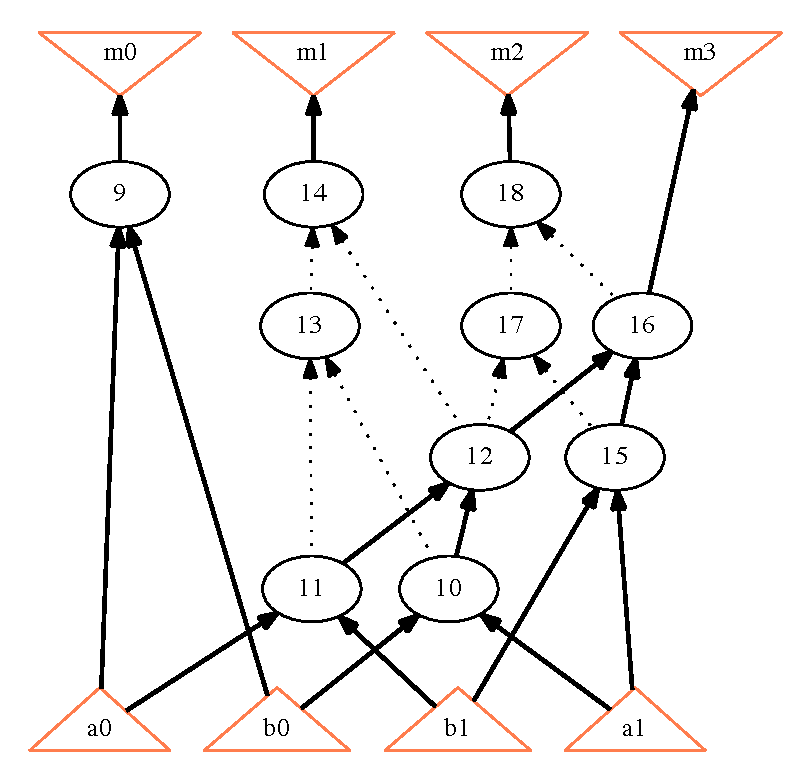
\includegraphics[scale=0.4]{../figs/2-bit-mult-aig.eps}
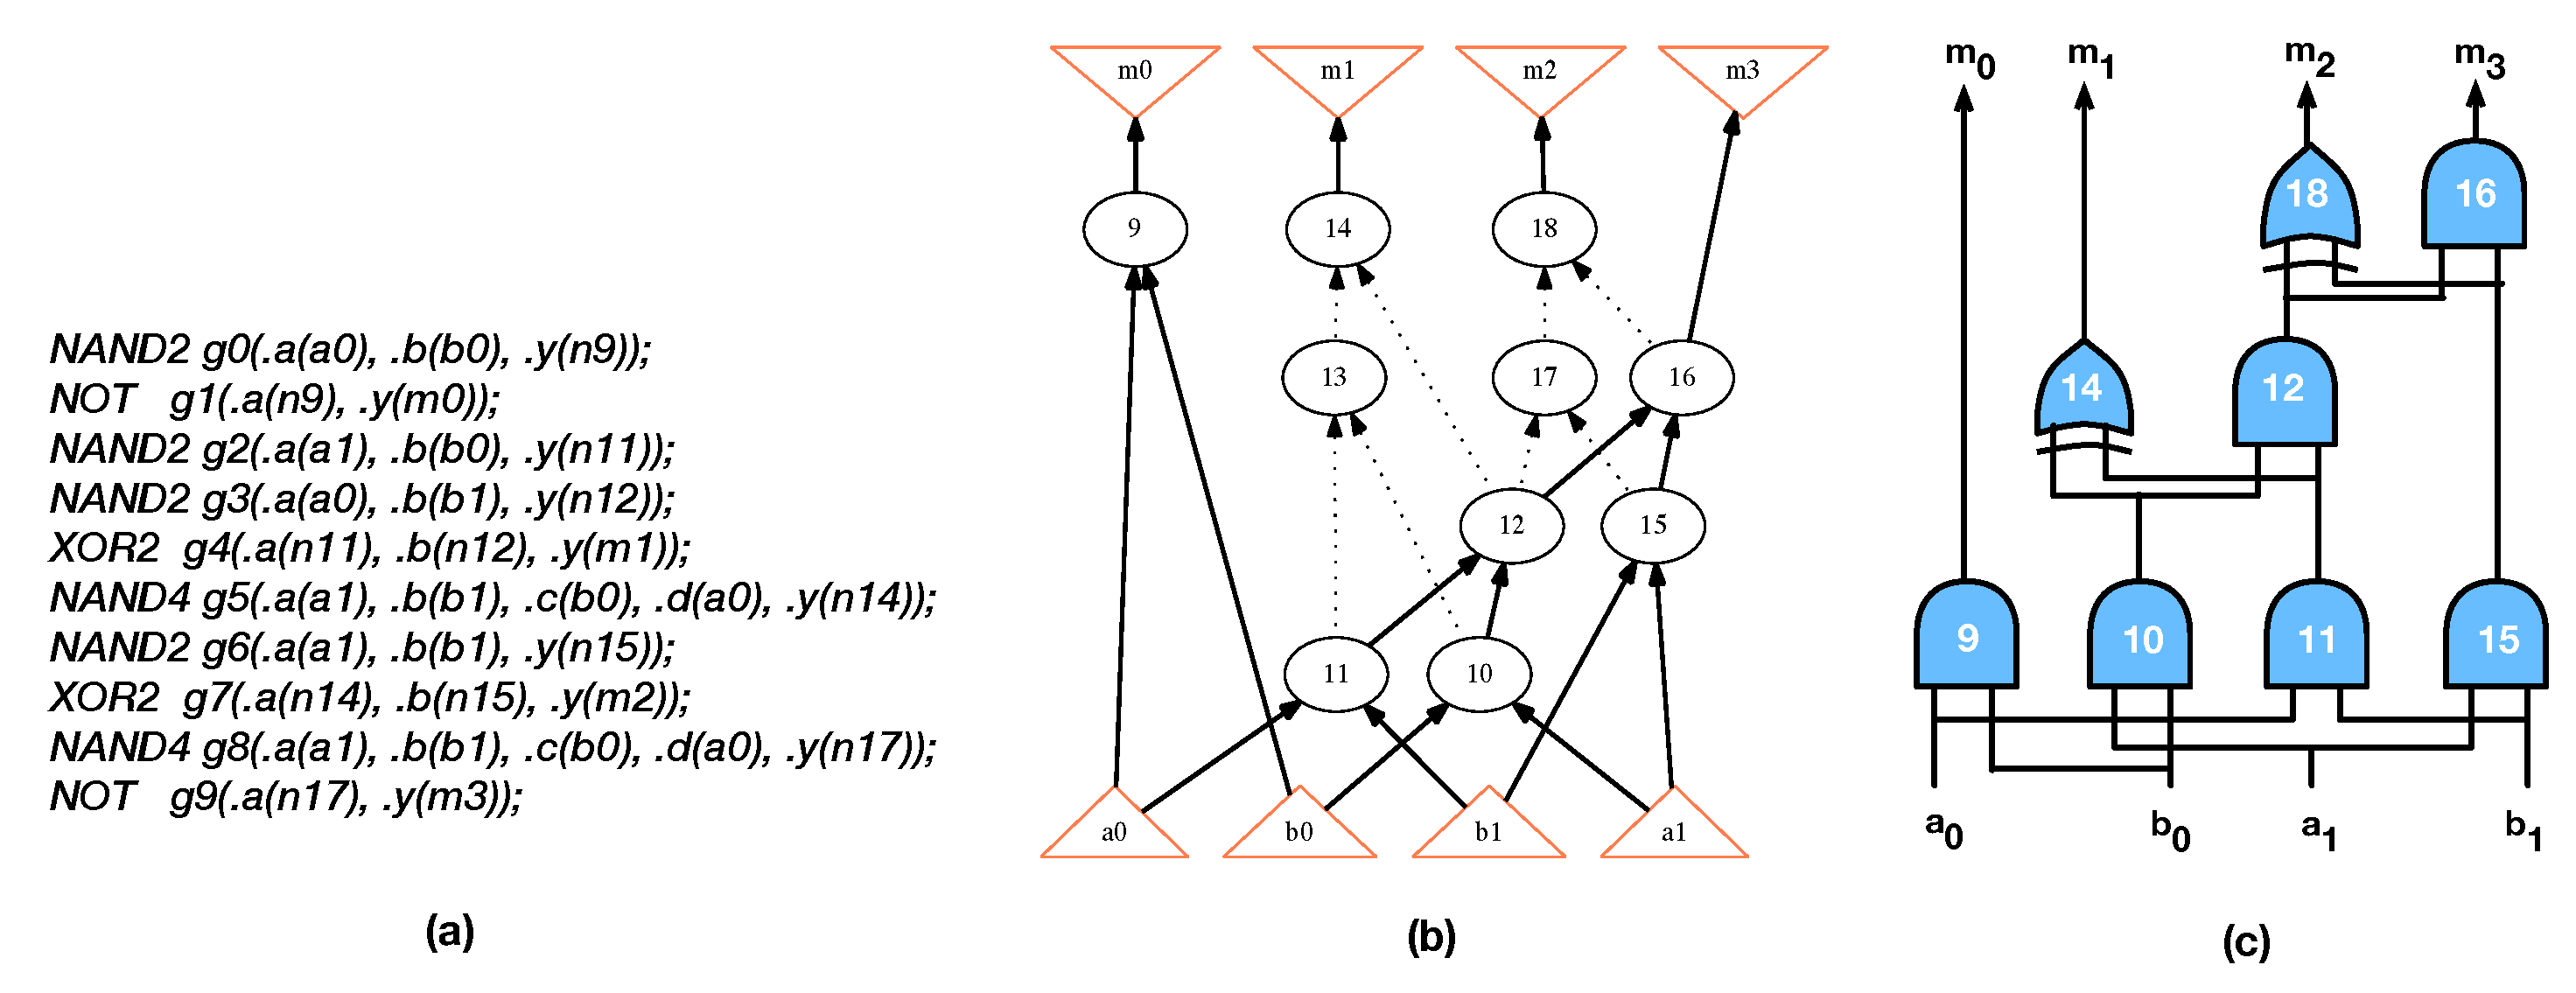
\includegraphics[scale=0.30]{../figs/aig-to-gatenetlist.eps}
\caption{(a) Post-synthesized 2-bit multiplier gate-level netlist; (b) The AIG of the 2-bit multiplier shown in Figure \ref{fig:2-bit-mult-aig}(a); (c) Detected unobserved functions from the AIG and the correspondences to AIG nodes. The index value in Figure \ref{fig:2-bit-mult-aig}(c) corresponds to the hash value of each node in Figure \ref{fig:2-bit-mult-aig}(b). }
\vspace{-3mm}
\label{fig:2-bit-mult-aig}
\end{center}
\end{figure*}

\section{Approach} \label{sec:approach}

This section presents the algebraic rewriting approach based on AIG. Similarly to \cite{ciesielski2015verification}, the algebraic rewriting process rewrites the output signature through all the nodes in the AIG in a topological order. As discussed in Section \rom{3}-E, the rewriting order that provides a large number of polynomial reductions, has significant impact on the performance of rewriting. However, there are many topological orders available in an AIG, since many nodes can have the same topological depth. This approach detects a topological order for algebraic rewriting that provides the maximum polynomial reductions. This is achieved by searching the pairs of MAJ3 and XOR3 nodes by computing the AIG \textit{Cuts}. 
%\begin{figure}[!htb] 
%\begin{center}
%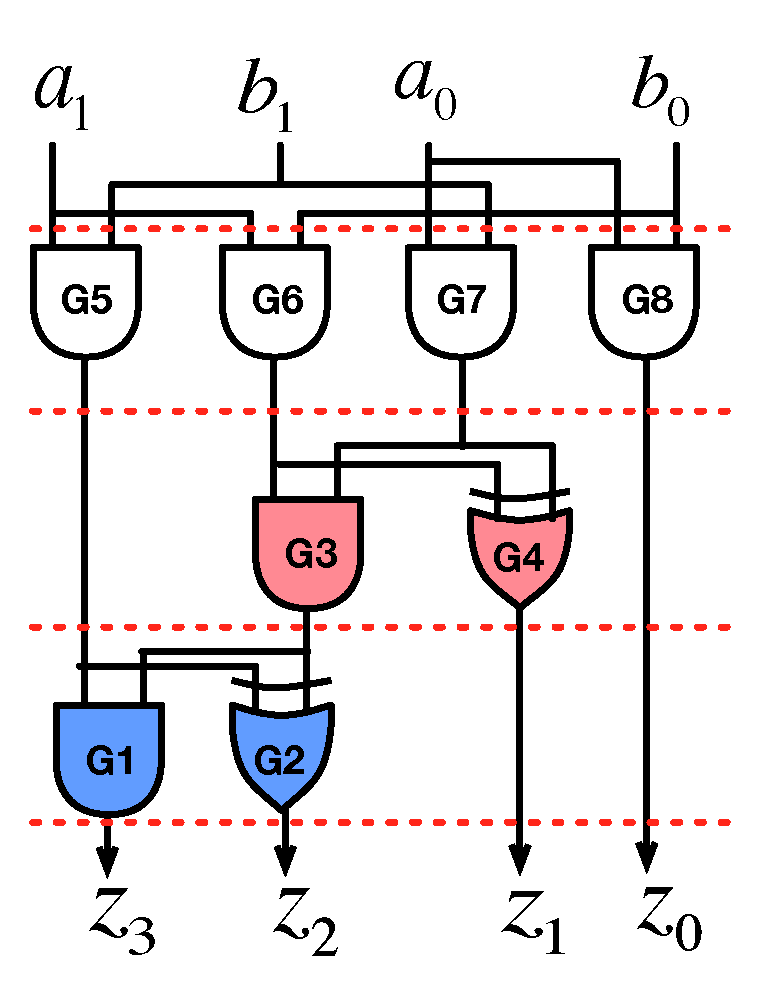
\includegraphics[scale=0.35]{../figs/order.eps}
%\caption{2-bit gate-level multiplier.}
%\label{fig:xor3-aig}
%\end{center}
%\end{figure}

\begin{algorithm}
\scriptsize
\caption{Algebraic Rewriting in AIG}\label{alg:algorithm}
\textbf{Input:} Gate-level netlist, output signature $Sig_{out}$  \\
\textbf{Output:} \textit{Pseudo-Boolean} expression extracted by rewriting 
\begin{algorithmic}[1]
\State Structural hashing the gate-level netlist into AIG, denoted \textit{G(V, E)}.
\State Detect all XOR3 and MAJ3 nodes in \textit{G(V, E)}.
\State Pair the XOR3 and MAJ3 if they have identical signals, denoted as $P$.
\State Topological sort \textit{G(V,E)} considering each element in $P$ as one node.
\State $i$ = 0; $F_{i}$ = $Sig_{out}$
\While{there are no elements remained in the topological order} %\Comment{We have the answer if r is 0}
\State Rewrite: $F_{i+1}$ = $F_{i}$ by substituting the variables with algebraic equations;
\State $i$ = i + 1
\EndWhile
\State \textbf{return} $F$ = $F_{i}$ (to be compared with $Sig_{in}$)
\end{algorithmic}
\end{algorithm}


\subsection{Outline of the Approach}

The proposed flow is outlined in Algorithm 1. The inputs to the algorithm are: the gate-level netlist and the output signature $Sig_{out}$. The flow includes three basic steps: 1) convert the gate-level implementation into AIG; 2) detect all pairs of XOR3 and MAJ3 nodes with identical inputs; topologically sort the AIG nodes while considering the detected pairs as one element; and 3) apply algebraic rewriting from POs to PIs following the topological order determined in step 2. Note that XOR2 and MAJ2(AND2) are the special cases of XOR3 and MAJ3, where one of the inputs is constant zero. The second step specifically processes as follows: 

\begin{itemize}

\item Compute all 3-feasible (3-input) cuts of all AIG nodes.

\item Compute truth tables of all cuts.

\item Store the cuts in the hash table by their ordered set of inputs.

\item Find pairs of 3-input cuts with identical inputs w.r.t to different nodes, such that the Boolean functions of the two cuts with the shared inputs are in \textit{NPN} classes of XOR3 and MAJ3, respectively.

\end{itemize}

Note that, in this approach, matching the XOR3 and MAJ3 nodes do not require the inputs and outputs polarity to be the same. Instead, all the cut-points are matched without considering the complement. For example, instead of being an exact XOR3, the function of a 3-feasible cut can be either XOR3 or XNOR3. Similarly, instead of being exactly MAJ3, the function of can be one of the eight functions forming the \textit{NPN} class of MAJ3 \cite{HuangWNM13}. To compute the cuts, the 3-input cut enumeration is performed in a topological order as described in \cite{PanL98}. The truth tables of the cuts are obtained as a by-product of the cut enumeration. Thus, when two fanin cuts are merged during the cut computation and the resulting cut is 3-feasible, the truth tables of fanin cuts are permuted to match the fanin order of the resulting cut. These truth tables are then ANDed or XORed, depending on the node type, to get the resulting truth table. For the case of 3-input cuts, a dedicated pre-computation reduces the runtime of truth table computation to a small fraction of that of cut enumeration.

%Moreover, when detecting the pairs of XOR3 and MAJ3 nodes, the algebraic coefficient of MAJ3 node is not required to be 2$\times$ of the coefficient of the XOR3 node. Although the non-linear terms reductions between those XOR3 and MAJ3 happen only if the coefficients satisfy this condition, there are significant polynomial reductions provided by the detected XOR3 and MAJ3 pairs. This is based on an important observation that the XOR3 and MAJ3 with identical inputs, are likely to construct a one-bit addition (full-adder or half-adder). 

As soon as the XOR3 and MAJ3 pairs are detected, algebraic rewriting will be applied to the AIG network in a constrained topological order, in which each XOR3 and MAJ3 pair is considered as one element. This means that at one topological depth, whenever either XOR3 or MAJ3 node of a pair (or its complement) is rewritten, the following rewriting element is of the other type. The AIG nodes with the same topological depth that do not exist in any pairs are ordered by their hashing value (in decreasing order). The algebraic rewriting ends when all elements in AIG network have been rewritten and the algorithm returns the extracted input signature. 


%\begin{figure}[t]
\scriptsize
\centering
\label{fig:2-bit-verilog}
\begin{tabular}{|l|}
\hline
\textit{\begin{tabular}[c]{@{}l@{}}and2 g0(.a(b0), .b(a0), .O(m0));\\ nand4 g1(.a(b1), .b(b0), .c(a1), .d(a0), .O(n10));\\ inv1 g2(.a(n10), .O(n11));\\ aoi22 g3(.a(b1), .b(a0), .c(b0), .d(a1), .O(n12));\\ nor2 g4(.a(n12), .b(n11), .O(m1));\\ and2 g5(.a(b1), .b(a1), .O(n14));\\ xnor2 g6(.a(n14), .b(n10), .O(m2));\\ nand4 g7(.a(b1), .b(b0), .c(a1), .d(a0), .O(n16));\\ inv1 g8(.a(n16), .O(m3));\end{tabular}} \\ \hline
\end{tabular}
\caption{Gate-level netlist of technology mapped 2-bit multiplier.}
\label{fig:2-bit-verilog}
\end{figure}





\textbf{Example 1 (2-bit CSA-multiplier):} The mapped gate-level netlist of a 2-bit CSA-multiplier is shown in Figure \ref{fig:2-bit-mult-aig}(a). First, the gate-level netlist is converted to an AIG representation (Figure \ref{fig:2-bit-mult-aig}(b)). Then, a set of XOR3 nodes $X$, and a set of MAJ3 nodes $M$ are detected. $X$ = \{\textit{14, 18}\}, $M$ = \{12, 16\}. \textit{Node 14} is \textit{XOR3(10, 11, 1'b0)} and \textit{node 12} is \textit{MAJ3(10, 11, 1'b0)}, where \textit{nodes 10 and 11} and constant zero \textit{1'b0} are the inputs; \textit{node 18} is \textit{XOR3(12, 15, 1'b0)} and \textit{node 16} is \textit{MAJ3(12, 15, 1'b0)}; \textit{1'b0} is Boolean \textit{false}. Hence, two pairs of XOR3 and MAJ3 are generated, \textit{(14, 12)} and \textit{(18, 16)}. The order of rewriting is determined as follows: 1) \textit{node 18} is the node with highest depth; it is detected as a XOR3 and paired with a MAJ3 \textit{node 16}; hence, the first rewriting starts from node 18 and 16, and ends at node 12 and 15; 2) similarly to the first rewriting, the second rewriting starts from nodes 14 and 12, and ends at nodes 11 and 10; 3) the remaining AIG nodes are ordered by their index value in decreasing order. The logic network after detecting all XOR3 and MAJ3 functions are shown in Figure \ref{fig:2-bit-mult-aig}(c). %The largest size of the internal polynomial expression of our approach is XX. [compared to the old approach here.] 


\subsection{Redundant Polynomial Determination}

In addition to the order of algebraic rewriting, identifying and using redundant polynomials could also provide significant polynomial reductions. For example, \textit{don't-care} polynomials and \textit{vanishing} polynomials are used for verifying sequential arithmetic circuits \cite{yu-isvlsi-16a}. Those polynomials are generated by observing that the signals that are removed for design efficiency contain algebraic information that is needed to cancel algebraic terms of the remaining output bits in the design. For example, the polynomial associated with the most significant bit (MSB) of an adder or a multiplier is such a polynomial. Such truncated designs are widely used in energy efficient applications by reducing critical paths and pruning the logic. However, automatically generating the redundant polynomials has not been adequately solved yet. 
%

%This is because MSBs of Booth multipliers are removed, i.e. the extra sign extension bits\footnote{A \textit{n}-bit Booth multiplier requires only \textit{2n} output bits. However, the Booth algorithm requires extra bits (sign extension) for intermediate computations. The number of extra bits added depends on the size of Booth encoding table.}. Those bits include a large number of algebraic monomials that can be used to reduce the size of internal polynomial during rewriting. In which case, they are considered as \textit{don't-care} polynomials. 

To efficiently apply algebraic rewriting to the multipliers with output bits truncated, an approach that automatically generates \textit{don't-care} polynomials is presented. This approach is based on an observation that the logic obtained by removing output bits is either a carry-out function or a sum function of one-bit addition. It is known that MAJ3 and XOR3 are the components that construct a 1-bit addition. Hence, using the approach of detecting pairs of XOR3 and MAJ3 (Section \rom{3}-A), the XOR3/MAJ3 nodes that do not belong to any such pair can be detected. For example, a $n$-bit CSA-multiplier with \textit{2n-1} output bits (with MSB removed), there is a missing MAJ3, i.e., the MAJ3s with identical inputs of an unpaired XOR3. Since one pair of XOR3 and MAJ3 constructs a 1-bit addition, removing the carry bit (MAJ3) makes the function an addition \textit{modulo 2}. In this case, the algebraic model of XOR3 (Equation 1) is reduced to \textit{a $\oplus$ b $\oplus$ c = a+b+c mod 2}. %The negation of the removed terms by modulo 2, $- 2ac - 2bc + 4abc$, gives the redundant polynomials detected for each unpaired XOR3. 

\textbf{Example 2 (3-bit CSA-multiplier with MSB $z_{5}$ detected):} The AIG after detecting XOR3 and MAJ3 pairs of a 3-bit post-synthesized CSA-multiplier with MSB deleted is shown in Figure \ref{fig:3-bit-aig}. The detected XOR3 and MAJ3 pairs are represented using the hash value of the root node of the XOR3 and MAJ3 nodes. We can see that there is one XOR3 (composed of two XOR2 nodes, \textit{41} and \textit{44}) with inputs $i_{36,37}$, $i_{27,29}$ and $i_{38}$, that cannot be paired with any MAJ3. This is because synthesis process removed the redundant logic (last carry out) while the MSB has been removed. In this case, the algebraic model of that XOR3 is reduced to $2^{4}$$\cdot$$z_{4}$($i_{49}$) = $2^4$$\cdot$($i_{36,37}$ + $i_{27,29}$ + $i_{38}$).



\begin{figure}[t] 
\begin{center}
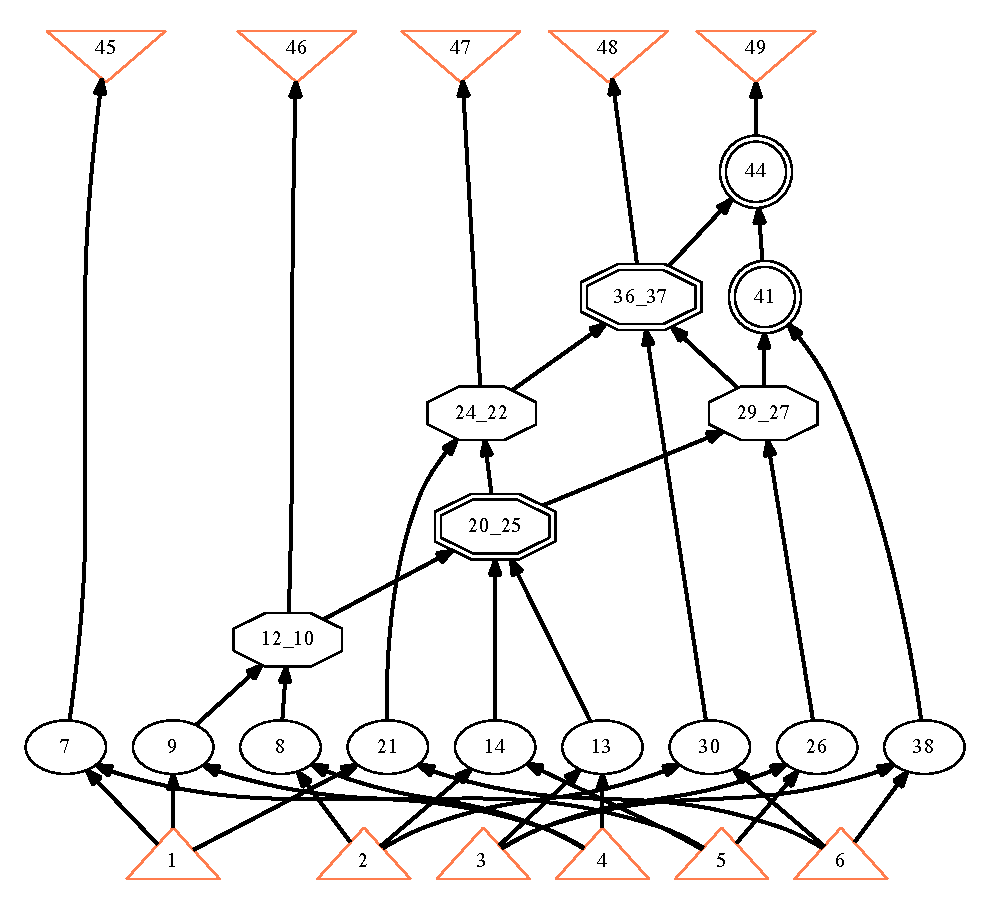
\includegraphics[scale=0.4]{../figs/truncate-mult3.eps}
\caption{Detecting \textit{MAJ3-XOR3} of a 3-bit post-synthesized CSA-multiplier with MSB $z_{5}$ deleted.}
\vspace{-3mm}
\label{fig:3-bit-aig}
\end{center}
\end{figure}












\section{Results}

The technique described in this paper was implemented in ABC \cite{abc-link}. It applies algebraic rewriting to the AIG and generates the polynomial signature. The experiments include gate-level rewriting of Carry-Save-Adder (CSA) multipliers up to 512 bits. The results are compared with \textit{functional extraction} \cite{ciesielski2015verification}.
The results show that the proposed technique is more efficient than the state-of-the-art technique for extracting the polynomial expressions for the CSA multipliers. The experiments were conducted on a PC with Intel(R) Xeon CPU E5-2420 v2 2.20 GHz x12 with 32 GB memory.

The results of applying AIG-based algebraic rewriting to pre-synthesized and post-synthesized CSA multipliers are shown in Table \ref{tbl:pre} and Table \ref{tbl:post}, respectively. The gate-level multipliers are taken from \cite{ciesielski2015verification}. Runtime and memory usage of \textit{functional extraction} \cite{ciesielski2015verification} are shown in columns 2 and 3, and the results of the proposed approach are shown in columns 4 and 5. The bit-width varies between 8 and 256 bits\footnote{512-bit post-synthesized multipliers are not reported in \cite{ciesielski2015verification}.}. First, we can see that the runtime of the proposing approach is lower than a second for both the pre- and post-synthesized CSA multipliers for any bit-width. At the same time, memory usage has been reduced on average 60\%, compared to \textit{function extraction} \cite{ciesielski2015verification}. Finally, the complexity of extracting the polynomial expression using functional extraction is increased when the multipliers are synthesized. For example, extracting post-synthesized 256-bit multiplier using functional extraction requires 9x more runtime and more memory. However, using the proposed approach, the runtime of extracting pre- or post-synthesized multipliers are almost the same.

% Please add the following required packages to your document preamble:
% \usepackage{multirow}
\begin{table}[t]
\centering
\caption{Results of applying AIG-based algebraic rewriting on pre-synthesized CSA-multipliers compared to \textit{function extraction} \cite{ciesielski2015verification}.}
\vspace{-1mm}
\label{tbl:pre}
\begin{tabular}{|r|r|r|r|r|}
\hline
\multirow{2}{*}{\# bits} & \multicolumn{2}{c|}{{[}1{]}} & \multicolumn{2}{c|}{This approach} \\ \cline{2-5} 
 & runtime(s) & mem(MB) & runtime(s) & mem(MB) \\ \hline
8 & 0.02 & 4.9 & 0.01 & 9.8 \\ \hline
16 & 0.10 & 8.2 & 0.01 & 10.4 \\ \hline
64 & 1.89 & 73.9 & 0.04 & 34.2 \\ \hline
128 & 8.12 & 288.4 & 0.15 & 117.2 \\ \hline
256 & 32.65 & 1157.3 & 0.82 & 440.5 \\ \hline
512 & 130.22 & 4427.5 & 3.76 & 1695.1 \\ \hline
\end{tabular}
\end{table}

\begin{table}[!htb]
\centering
\caption{Results of applying AIG-based algebraic rewriting to post-synthesized CSA-multipliers compared to \textit{functional extraction} \cite{ciesielski2015verification}.}
\label{tbl:post}
\begin{tabular}{|r|r|r|r|r|}
\hline
\multirow{2}{*}{\# bits} & \multicolumn{2}{c|}{{[}1{]}} & \multicolumn{2}{c|}{This approach} \\ \cline{2-5} 
 & runtime(s) & mem(MB) & runtime(s) & mem(MB) \\ \hline
8 & 0.04 & 2.9 & 0.01 & 9.7 \\ \hline
16 & 0.14 & 6.1 & 0.01 & 10.4 \\ \hline
64 & 5.50 & 76.3 & 0.04 & 34.3 \\ \hline
128 & 39.64 & 299.2 & 0.16 & 120.0 \\ \hline
256 & 285.22 & 1250.6 & 0.82 & 438.9 \\ \hline
\end{tabular}
\end{table}

%% Please add the following required packages to your document preamble:
% \usepackage{multirow}
\begin{table}[]
\centering
\caption{My caption}
\label{my-label}
\begin{tabular}{|r|r|r|r|r|}
\hline
\multirow{2}{*}{n-bit} & \multicolumn{2}{r|}{{[}1{]}} & \multicolumn{2}{r|}{This approach} \\ \cline{2-5} 
 & runtime(s) & mem(MB) & runtime(s) & mem(MB) \\ \hline
16 &  &  &  &  \\ \hline
32 &  &  &  &  \\ \hline
64 &  &  &  &  \\ \hline
128 &  &  &  &  \\ \hline
256 &  &  &  &  \\ \hline
512 &  &  &  &  \\ \hline
\end{tabular}
\end{table}


\maketitle

\IEEEdisplaynontitleabstractindextext

\IEEEpeerreviewmaketitle

\vspace{-3mm}

\section{Conclusion}
This paper presented a method to improve the efficiency of algebraic rewriting used in arithmetic verification. The method is based on the representation of the Boolean network called an And-Inverter Graph (AIG). This approach allows for formal verification of practical multipliers that are heavily optimized and mapped using 14nm technology library. Another contribution of the paper is a technique that automatically detects redundant polynomials to reduce the complexity of algebraic rewriting.


\section*{Acknowledgment}
This work was supported by an award from National Science Foundation, No. CCF-1319496 and No. CCF-1617708. The co-author affiliated with UC Berkeley was supported in part by NSA grant ``Enhanced equivalence checking in
crypto-analytic applications''.



\bibliographystyle{IEEEtran}
\bibliography{/Users/cunxiyu/Documents/Texshop/cunxi_bib/verification_ycunxi,/Users/cunxiyu/Documents/Texshop/cunxi_bib/synthesis}

\end{document}

